\documentclass[10pt,letterpaper]{article}
\usepackage[margin=.82in]{geometry}
\usepackage[T1]{fontenc}\usepackage{lmodern,graphicx,booktabs,amsmath,xcolor,hyperref,xurl,caption,fancyhdr}
\hypersetup{colorlinks=true,urlcolor=teal,linkcolor=teal,pdftitle={Check a solar-resource shortlist before treating it as a project shortlist},pdfauthor={James Jean}}
\pagestyle{fancy}\fancyhf{}\fancyhead[L]{\small Solar resource shortlist / Study 29}\fancyhead[R]{\small Independent retrospective study}\fancyfoot[C]{\thepage}
\setlength{\headheight}{14pt}\setlength{\parindent}{0pt}\setlength{\parskip}{6pt}\captionsetup{font=small,labelfont=bf,hypcap=false}
\begin{document}
{\small\color{teal} SOLAR RESOURCE SCREENING / RANKING AND COVERAGE\par}
\vspace{7pt}{\LARGE\bfseries Check a solar-resource shortlist\par}\vspace{4pt}{\large Year-to-year variation and missing-day sensitivity\par}
\vspace{6pt}James Jean \hfill 30 October 2026
\section*{The decision}
A resource shortlist should show whether small ranking differences survive year-to-year variation and gaps in the source record. This study compares six simple historical-resource rules at twelve fixed Southwest grid locations, then deliberately removes daily blocks to inspect sensitivity. The output is a transparent screening review, with no plant output or financial return estimate.

\textbf{Finding.} The development-selected ten-year mean rule has held mean two-point shortlist regret of \textbf{0.000000} in the western cohort and \textbf{0.005710} in the eastern cohort, in kWh/m$^2$/day. All six rules choose the best western pair in every held year; several rules share the same eastern shortlist score. The selected rule has no demonstrated unique decision advantage.

\textbf{Coverage matters near a boundary.} Removing a thirty-day block at each month start changes \textbf{4/84 western} and \textbf{6/84 eastern} shortlists. Mean absolute resource bias is 0.144269 and 0.134706 kWh/m$^2$/day, respectively. These are fixed artificial removals from complete records, not estimated frequencies of satellite data loss.

\begin{center}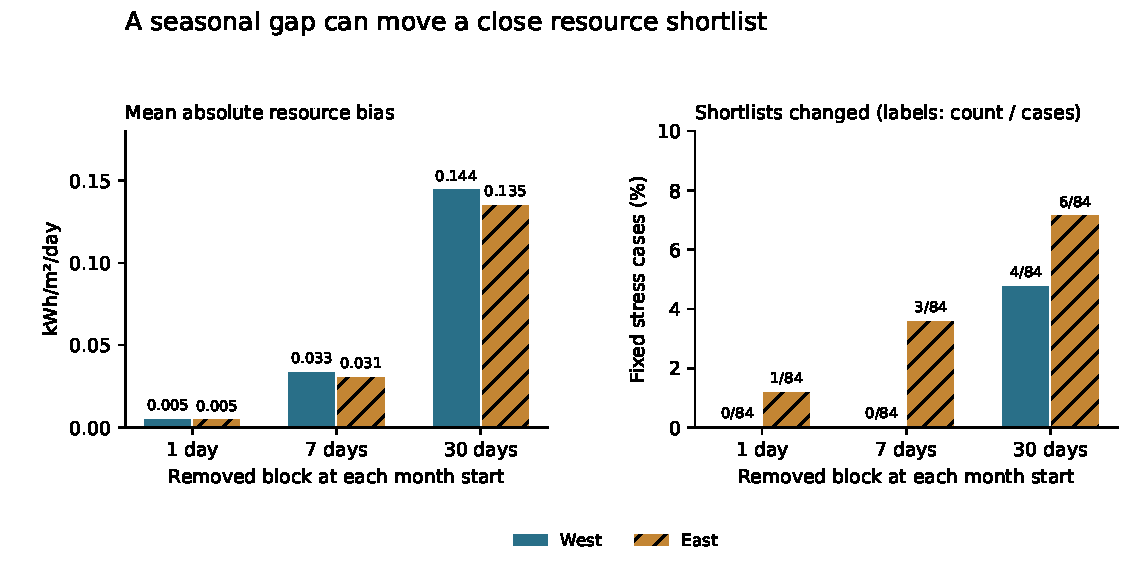
\includegraphics[width=\linewidth]{images/missing_day_sensitivity.pdf}\end{center}
\captionof{figure}{Each duration has seven held years times twelve month starts per cohort. The same block is removed from all six points within a case. Scenarios share source records and are not independent replications.}

\textbf{Practical next step.} Review the close alternatives and data coverage before treating a ranking as actionable. Obtain finer site measurements, land and connection constraints, system design, costs and tariffs for a real project. NASA's gridded radiation estimates do not establish parcel suitability or realized generation.
\newpage
\section*{1. Source, coordinates and the unit check}
The historical proposal named NSRDB; its convenient per-point API requires an API key and active email [1]. No new account or credential was created. This implementation explicitly uses NASA Langley POWER's public Daily API instead [2--4]. It is a different source and is identified as such in the repository. POWER supplies satellite-and-model estimates; it does not provide twelve newly measured ground stations.

The fixed points are the Cartesian products of latitudes 32.5, 34.5 and 36.5 degrees with western longitudes $-114.5,-112.5$ and eastern longitudes $-108.5,-106.5$. These are deliberately chosen examples, not an existing project shortlist or a probability sample. The official primary solar source uses a one-degree grid. Returned coordinates match requests; plotted cell boxes derive from that documented resolution. The API does not return an independently audited internal cell ID, and no spatial independence is assumed.

\begin{center}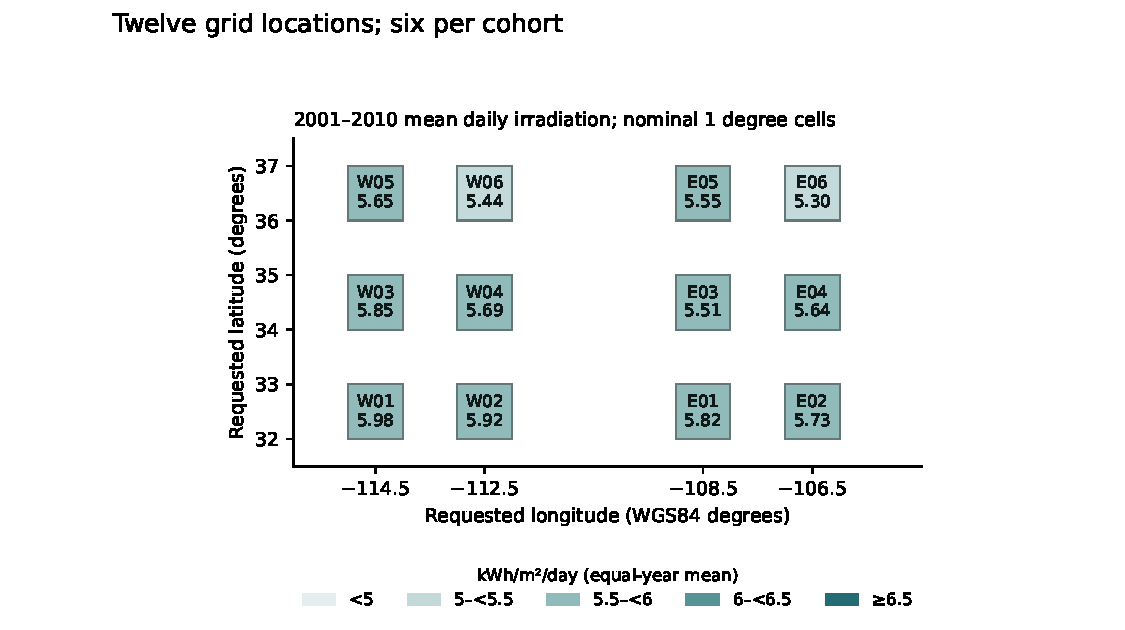
\includegraphics[width=\linewidth]{images/grid_resource.pdf}\end{center}
\captionof{figure}{The twelve requested locations and initial ten-year equal-year mean daily irradiation. Boxes illustrate nominal one-degree cells, with no interpolation or parcel boundary claim. Color bins are fixed and labels show values. The gap between cohorts does not establish independent weather errors.}

The precollection protocol was committed at \texttt{d90e7cb}; the exact request/capture code at \texttt{8413e7b}. Twenty-four JSON/CSV responses were captured once, sequentially, for 2001--2023, with UTC times, HTTP status, relevant headers, bytes and SHA-256 before parsing. The source projection has 100,800 daily rows, 8,400 per point. All 276 point-years are complete, and all twelve points pass the fixed annual/monthly coverage gate. No identical complete series alias is observed.

\textbf{Returned units differed from the anticipated community unit.} Daily API v2.10.1 returns daily mean irradiance in W/m$^2$, with source SYN1DEG and UTC. After inspecting the schema and the first five daily values at W01, but before annual qualification or ranking, \texttt{UNIT\_BINDING.md} documented the conversion permitted by the protocol: daily irradiation equals daily mean W/m$^2$ times 24 hours divided by 1,000. Both native values and exact converted fractions remain available. This is unit integration, not photovoltaic modeling or an untouched source-unit preregistration.
\newpage
\section*{2. Fixed information boundary and development choice}
A point-year qualifies at at least 99\% valid daily values and at least 95\% in every month. Source fill and invalid values remain unavailable, never zero. A point must qualify in every year; each cohort needs at least four distinct requested source-cell series. All six points per cohort qualify. The annual resource is the mean available daily irradiation, not an imputed annual total. An independent SQL/Decimal reconstruction checks 19,451 calendar, coverage and input conditions.

For target year $Y$, a rule uses only annual values at that location from years before $Y$. Candidates are last year, trailing means over three/five/ten years, trailing ten-year median and the nearest-rank twentieth percentile over ten years. The quantile is the second ordered value of ten. Windows and quantile are declared diagnostics; there is no learned estimator. Current retrieved historical estimates do not prove original publication vintages or exact-day access. Later held years may use earlier held outcomes as rolling history, with no retuning.

Within a cohort, select the two largest predicted resources. Exact ties prefer ascending point ID; full rankings, tied boundary sets and midranks are exported. The target-year best pair is an oracle used only for scoring. For selected set $S_Y$ and oracle $O_Y$, regret is
\[
 R_Y=\tfrac12\sum_{i\in O_Y}x_{iY}-\tfrac12\sum_{i\in S_Y}x_{iY},
\]
in kWh/m$^2$/day. Also retain all-point MAE, overlap with the oracle pair and Spearman correlation with midranks. Undefined constant-vector correlations remain unknown. Correlations are displayed to nine decimals, then their displayed annual values are averaged; exact gain/error/regret calculations retain fractions. Decimal display is not physical measurement precision.

\begin{center}\small\begin{tabular}{lrrr}\toprule
Western development, 2011--2016 & Mean regret & All-point MAE & Pair overlap (\%)\\\midrule
Last year & 0.015607 & 0.068953 & 83.3 \\
Mean 3 years & 0.005163 & 0.054657 & 91.7 \\
Mean 5 years & 0.005163 & 0.054295 & 91.7 \\
Mean 10 years* & 0.005163 & 0.051642 & 91.7 \\
Median 10 years & 0.005163 & 0.052497 & 91.7 \\
Q20 over 10 years & 0.005163 & 0.072128 & 91.7 \\
\bottomrule\end{tabular}\end{center}
Select mean annual regret, then all-point MAE, then the fixed candidate order. Five candidates tie on regret. Mean ten years wins the declared MAE tie-break; it is not uniquely best at shortlisting. All six candidates remain in the release. No eastern ranking outcome is used for selection. Earlier eastern local resource is allowed as input history, so the later comparison is geographic transfer with local history.

Twenty-eight source/code/development dependency hashes were committed at \texttt{97276d1} before 2017--2023 held summaries in both cohorts. Separate hashes for the fixed missing-day implementation, checker, fixtures and original freeze manifest were committed at \texttt{b6df76b} before any stress output. No held outcome changes a candidate, location, gate, objective, tie convention or removal schedule. Held years are serially related and input windows overlap; no independent-trial or significance claim is made.
\newpage
\section*{3. Held forecasts: similar decisions can hide different errors}
Each cohort contains six fixed points and seven held years. Regret and MAE are in kWh/m$^2$/day; overlap is the fraction of the oracle's two canonical points retained, averaged across years. Source estimates define the comparison target; they are not independent site truth.
\begin{center}\small\begin{tabular}{llrrr}\toprule
Cohort & Rule & Mean regret & All-point MAE & Pair overlap (\%)\\\midrule
West & Last year & 0.000000 & 0.105324 & 100.0 \\
 & Mean 3 years & 0.000000 & 0.081787 & 100.0 \\
 & Mean 5 years & 0.000000 & 0.070974 & 100.0 \\
 & Mean 10 years* & 0.000000 & 0.063264 & 100.0 \\
 & Median 10 years & 0.000000 & 0.062065 & 100.0 \\
 & Q20 over 10 years & 0.000000 & 0.075248 & 100.0 \\
East & Last year & 0.022373 & 0.098910 & 71.4 \\
 & Mean 3 years & 0.017327 & 0.085820 & 71.4 \\
 & Mean 5 years & 0.005710 & 0.068806 & 78.6 \\
 & Mean 10 years* & 0.005710 & 0.063032 & 78.6 \\
 & Median 10 years & 0.005710 & 0.064900 & 78.6 \\
 & Q20 over 10 years & 0.005710 & 0.114897 & 78.6 \\
\bottomrule\end{tabular}\end{center}
\begin{center}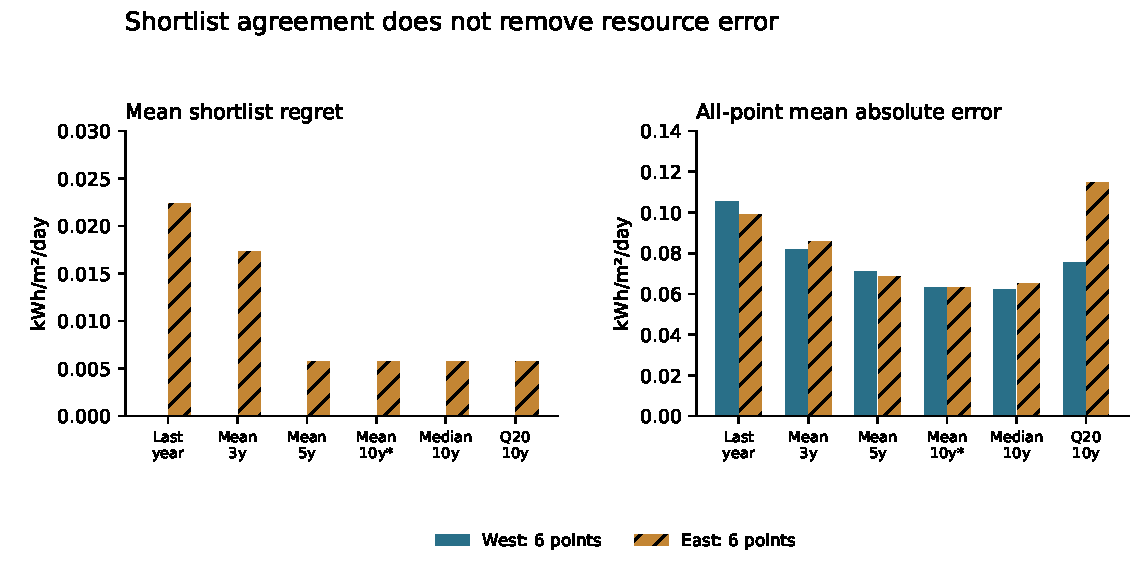
\includegraphics[width=\linewidth]{images/held_resource_errors.pdf}\end{center}
\captionof{figure}{Asterisk marks the frozen development choice. All western regrets are zero, while point errors differ. Four rules tie on eastern regret. The lower-quantile rule is a conservative resource score, not a fitted conditional-mean forecast.}

The western median has slightly lower held MAE than the selected ten-year mean; the frozen choice is retained. In the east, mean five, mean ten, median ten and Q20 have identical shortlist scores. Q20 nevertheless has a larger point MAE than persistence. This distinction matters when a user needs both a resource estimate and a ranking: one metric cannot certify the other. The positive observations are bounded to these locations and years; no future shortlist success, source-accuracy improvement or new forecasting method is established.
\newpage
\section*{4. Missing-day cases: seasonal bias and close alternatives}
Actual captured coverage is complete. To test a fixed failure mechanism, remove a contiguous block of one, seven or thirty days starting on the first day of each month, without wrapping across year-end. Recompute the mean from remaining daily values and compare it with the intact mean. The common calendar block applies to every point in that cohort/year, rather than allowing an analyst to choose a favorable point-specific gap.

The complete stress export has 3,024 point cases and 504 cohort shortlists. For each duration/cohort, 504 point cases feed mean/max bias and 84 shortlist cases feed choice changes. These repeated scenarios share data, so the counts are not independent observations or probabilities of future missingness. Intact-mean regret scores the gap-induced pair using the intact resource, not the incomplete average.
\begin{center}\small\begin{tabular}{llrrrr}\toprule
Cohort & Days & Changed / cases & Mean abs. bias & Max abs. bias & Intact regret\\\midrule
West & 1 & 0/84 & 0.004925 & 0.014136 & 0.000000 \\
 & 7 & 0/84 & 0.033486 & 0.072137 & 0.000000 \\
 & 30 & 4/84 & 0.144269 & 0.290219 & 0.000395 \\
East & 1 & 1/84 & 0.004626 & 0.013239 & 0.000011 \\
 & 7 & 3/84 & 0.030619 & 0.070130 & 0.000034 \\
 & 30 & 6/84 & 0.134706 & 0.289753 & 0.000241 \\
\bottomrule\end{tabular}\end{center}
\begin{center}\small\begin{tabular}{rrrrr}\toprule
Year & West changed & West bias & East changed & East bias\\\midrule
2017 & 0/12 & 0.1482 & 0/12 & 0.1350 \\
2018 & 0/12 & 0.1477 & 5/12 & 0.1404 \\
2019 & 0/12 & 0.1465 & 0/12 & 0.1331 \\
2020 & 4/12 & 0.1497 & 0/12 & 0.1395 \\
2021 & 0/12 & 0.1367 & 0/12 & 0.1255 \\
2022 & 0/12 & 0.1339 & 1/12 & 0.1292 \\
2023 & 0/12 & 0.1472 & 0/12 & 0.1403 \\
\bottomrule\end{tabular}\end{center}
The annual table uses thirty-day blocks, twelve month starts per year; bias is mean absolute kWh/m$^2$/day across points and starts. The eastern one-day removal changes one shortlist despite a small average bias. A large annual-average error is therefore not required for a near-boundary ranking change. Conversely, many gaps move resource levels without changing the selected pair. Neither observation establishes an actual outage mechanism.

\textbf{What remains unknown.} This bounded grid example does not resolve local shading, terrain, sub-grid cloud variation, land rights, interconnection, system tilt, temperature, inverter loss, storage, costs or tariffs. POWER's source documentation identifies current CERES SYN1deg and notes multiple product streams and edition-specific validation. Restricting to 2001--2023 avoids the stated pre-2001 SRB transition and current low-latency tail, but does not prove a homogeneous climate record or justify a causal climate-trend claim. No independent ground-station validation is performed. Nominal grid separation does not establish independent spatial errors.
\newpage
\section*{5. Implementation, reproduction and source attribution}
\textbf{A useful exercise.} Pick an eastern held year with a changed pair. Reconstruct the six candidates from strictly earlier annual values and inspect the full tied score sets. Then select a reported missing-day case and recompute its remaining-day denominator, resource bias and pair. Explain what evidence is missing before a physical project can be chosen. Do not add a hypothetical tariff or multiply radiation by an invented capacity and report it as measured electricity.

\textbf{Evidence.} Independent Pandas/SQLite decoding checks 806,558 original-source conditions; source projection uses separate CSV/JSON parsers and preserves every planned date. Independent qualification, development and held reconstruction checks 19,451, 3,394 and 7,884 conditions, respectively. A separate native-flux/ordinal-date checker verifies 41,886 stress conditions. These are scalar/structural checks, not that many physical observations. Thirty-five finite fixtures include calendar/coverage boundaries, null versus zero, aliases, exact ties, quantiles, constant correlations, unit mismatch and year-end removals; they do not prove universal correctness.

Run \texttt{python src/reproduce.py} from a full-history checkout. Original-preserving replay passes locally with Python 3.10 and 3.12.14, rebuilding separate temporary outputs and matching 96,847 CSV fields including headers and six JSON documents. It preserves the original frozen files, checks both dependency manifests, runs independent arithmetic and fixtures, and makes no new source requests. Public source checks verify the retained projection hash/count; private-original decoding additionally needs the retained response files. The figure checker reconstructs 48 values, 384 actual SVG coordinates, twelve map colors and nine hashes. The paper checker independently verifies every ledgered numerical display and scoped file hash. Three figures and all rendered manuscript pages are inspected separately.

\textbf{Attribution and rights.} Data are from NASA Langley Research Center's POWER project, funded through NASA Earth Science Division, Daily API v2.10.1, accessed 30 October 2026. Minimal factual radiation values, request lineage and new calculations are retained; original responses, source pages and unused contact metadata stay private. NASA's science-data policy distinguishes marked terms, NASA-led mission data and other as-is data [5]. No restrictive notice appears in the captured responses; no blanket right to logos, source text or unrelated third-party products is claimed. POWER requests publication/redistribution notification [4]; no unsolicited email is sent by this study. NASA does not endorse these choices. This independent program manuscript is not peer reviewed. Formal-publication projects, including Azure optimization, remain private.

\small
[1] NLR, \emph{NSRDB Data Download Usage Guide}. \url{https://developer.nlr.gov/docs/solar/nsrdb/guide/}.

[2] NASA POWER, \emph{Daily API}; daily means, time standards and formats. \url{https://power.larc.nasa.gov/docs/services/api/temporal/daily/}.

[3] NASA POWER, \emph{Energy Fluxes: Data Sources and Validation}. \url{https://power.larc.nasa.gov/docs/methodology/data/sources_fluxes/}. Also NLR, \emph{Solar Resource Glossary}: \url{https://www.nlr.gov/grid/solar-resource/solar-glossary}.

[4] NASA POWER, \emph{Referencing Guide}. \url{https://power.larc.nasa.gov/docs/referencing/}. Exact request URLs, response/source metadata, access times and hashes are in the repository manifest.

[5] NASA, \emph{Science Data Licenses}. \url{https://science.data.nasa.gov/about/license}. Official documentation was checked before scoring; source-page captures and receipts are privately retained.
\end{document}
